\documentclass[11pt]{article}
\textwidth 16.5cm               
\textheight 25.5cm
\oddsidemargin -0.0cm
\evensidemargin -0.7cm
\topmargin -1.5cm
\headheight 0cm
\headsep 0.9cm
\usepackage{graphicx}
\usepackage{pstricks,pst-plot,pst-node,pst-text}
\usepackage{marvosym}
\usepackage{endnotes}
\usepackage{pslatex}
\usepackage{apacite}
\usepackage{amssymb}
\usepackage{rotating}
\usepackage{verbatim}
\title{Experiments on Aristotle's Thesis:\\ Towards an experimental
  philosophy of conditionals}
\author{Niki Pfeifer ({\tt niki.pfeifer@lrz.uni-muenchen.de})}
\date{Munich Center for Mathematical Philosophy, Ludwig-Maximilians-Universit\"at M\"unchen\\
  Hauspost Fach 90, Geschwister-Scholl-Platz 1, 80539 Munich, Germany}
\renewcommand{\baselinestretch}{2}
\begin{document}

\maketitle

\renewcommand{\footnote}{\endnote}




\begin{abstract}
  Two experiments ($N_1=141$, $N_2=40$) investigate two versions of
  Aristotle's Thesis for the first time. Aristotle's Thesis is a
  negated conditional, which consists of one propositional variable
  with a negation either in the antecedent (version~1) or in the
  consequent (version~2). This task allows to infer if people
  interpret indicative conditionals as material conditionals or as
  conditional events.  In the first experiment I investigate
  between-participants the two versions of Aristotle's Thesis crossed
  with abstract versus concrete task material. The modal response for
  all four groups is consistent with the conditional event and
  inconsistent with the material conditional interpretation. This
  observation is replicated in the second experiment. Moreover, the
  second experiment rules out scope ambiguities of the negation of
  conditionals. Both experiments provide new evidence against the
  material conditional interpretation of conditionals and support the
  conditional event interpretation. Finally, I discuss implications
  for modeling indicative conditionals and the relevance of this work for
  experimental philosophy.

\textbf{Keywords:}
experimental philosophy; conditionals; probability; negation

\end{abstract}
\section{Introduction}


Experimental philosophers investigated people's intuitions already on
a wide variety of philosophical topics, including causation,
consciousness, cross-cultural intuitions, epistemology, morality, free
will, and intentional action \cite<see,
e.g.,>{xphipage,knobe08,feltz09}. Conditionals, however, have not been
discussed by experimental philosophers yet. This paper aims to extend
the domain of experimental philosophy to conditionals. After a brief
review of philosophical and psychological intuitions on probabilistic
interpretation of indicative  conditionals, I report two new experiments on reasoning
about conditionals to clarify the interpretation and negation of
indicative conditionals.


There is a long tradition of  psychological investigations of
conditionals. Standard tasks include Wason's selection task, truth
table tasks, and conditional elimination tasks \cite<like modus
ponens; see, e.g.,>{evans93}. The propositional calculus was taken for
granted as \emph{the} rationality norm: rational inferences are
consistent with the laws of logic and indicative conditionals (of the
form ``If $A$, then $B$'') should be interpreted as material
conditionals (denoted by $A\supset B$). People's inferences, however,
diverged from the rationality postulates of classical logic.

Philosophers argued for  probabilistic interpretations of indicative
conditionals  by
relating conditionals to  conditional probability, $P(B|A)$ \cite<e.g.,>{adams75,bennett03,douven08,ramsey26}. The argument of the
conditional probability function is the conditional event $B|A$. The
conditional event cannot be captured within the framework of classical
logic. Contrary to the material conditional ($A\supset B$) and the
conjunction ($A\wedge B$), the conditional event cannot be expressed
by any Boolean function: the conditional event is \emph{void}, if the
antecedent ($A$) is false (see Table~\ref{tt}).



\dotfill

\dotfill \emph{insert Table
\ref{tt} about here} \dotfill

\dotfill



There
are striking \emph{a priori} reasons, why indicative conditionals are
not material ones. As an example, imagine that
Jones ``is about to be dealt a five card poker
hand from a shuffled deck of 52 cards'' \cite[p.~1]{adams05}. Someone asserts:
\begin{center}
\fbox{If Jones's first card is an ace, then Jones's second card is an ace.}
\end{center}
\noindent
How sure can you be, that the sentence in the box holds? If you
interpret the sentence as a conditional event and assign a conditional
probability, you obtain a very low probability value\footnote{Of all
  52 cards only four ones are aces. If the first card is an
  ace, three aces are left for drawing a second ace out of the 51
  remaining cards. Thus,
  $P(\mbox{Jones's second card is an ace}\, |\, \mbox{Jones's first
    card is an ace})= 3/51\simeq 0.06$.}, which is intuitively
plausible, \[P(\mbox{Jones's second card is an ace}\, |\,
\mbox{Jones's first card is an ace})= \frac{3}{51} \simeq 0.06\, .\]

\noindent
If you interpret the sentence in the box as a material conditional,
you obtain in this scenario an intuitively implausible high
probability value\footnote{Let ``$A$'' denote the antecedent and
  ``$B$'' denote the
  consequent of the conditional. $P(A\supset B)=1-P(A\wedge \neg B)=1-\left(\frac{4}{52}\times
  \frac{48}{51}\right)=\frac{205}{221}\simeq 0.93$.},

\[P(\mbox{Jones's first card is an ace}\,  \supset \,
    \mbox{Jones's second card is an ace})= \frac{205}{221}\simeq 0.93\, .\]



    \noindent Some of the arguments in favor of the conditional event
    interpretation have been confirmed empirically. Contrary to the
    material conditional, the conditional event interpretation avoids
    the paradoxes of the material conditional and people do not endorse
    these paradoxes \cite{pfeifer10b}. Premise strengthening and
    contraposition do not hold under the conditional event
    interpretation and people do not endorse these argument forms
    \cite{pfeifer10a}.

    In recent years, probabilistic rationality norms emerged in the
    psychology of reasoning to better deal with the defeasibility and
    uncertainty and to match closer everyday inference
    \cite<e.g.,>{evans04,oaksford09a,pfeifer05a,pfeifer09b}. Within
    these probabilistic approaches, a new hypothesis concerning the
    interpretation of conditionals emerged: people interpret
    indicative conditionals (If $A$, then $B$) as conditional events
    ($B|A$). Recent studies \cite<e.g.,>{fugard11,fugardip,oberauer06,over07b}
    provide strong empirical evidence for this hypothesis. 



    The present paper further investigates the conditional event
    hypothesis. Specifically, it investigates two versions of
    Aristotle's Thesis for the first time. Aristotle's Thesis is a
    negated conditional, which consists of one propositional variable
    with a negation either in the antecedent (version~1) or in the
    consequent (version~2):




\begin{tabular}{ll}
(AT~\#1)& $\neg (\neg A\rightarrow A)$ \\
(AT~\#2) & $\neg (A\rightarrow \neg A)$\\
\end{tabular}

\noindent ``$\neg$'' denotes negation.\footnote{The name ``Aristotle's
  Thesis'' was coined by \citeA{mccall66}. Aristotle wrote in his
  \emph{Prior Anlaytics} ``\dots if $B$ is not great, $B$ itself is
  great. But this is impossible.'' \cite<quoted
  after>[p.~50]{lukasiewicz57}.} ``$A \rightarrow B$'' denotes the
indicative conditional \emph{If $A$, then $B$}, where the semantics of
$\rightarrow$ is not specified.  AT~\#1 and AT~\#2 are intuitively
plausible. Consider an instance in natural language:
\begin{quote}
It is not
the case that: If I do not win the lottery, then I win the
lottery.
\end{quote}
\noindent
Likewise, it is plausible to assert
\begin{quote}
It is not the case
that: If I win the lottery, then I do not win the lottery.
\end{quote}


In classical logic, where ``$\rightarrow$'' is interpreted as a
material conditional, (AT~\#1) and (AT~\#2) are not theorems. Both
formulas are contingent (``$\equiv$'' denotes equivalence):

\[\neg ( \neg A \supset A) \quad \equiv\quad \neg A \wedge \neg
  A\quad \equiv\quad \neg A \]
\[ \neg (A\supset \neg A) \quad \equiv\quad A \wedge A \quad \equiv\quad A\]

In this paper, I propose an interpretation that justifies the
rationality of high beliefs in AT~\#1 and AT~\#2. Specifically, I
formalize AT in terms of coherence based probability logic
\cite{pfeifer06d,pfeifer09b}.

In the psychology of reasoning three interpretations of indicative
conditionals (If $A$, then $B$) are currently debated: the conditional
event interpretation ($P(B|A)$), the material conditional
interpretation ($P(A\supset B)$), and the conjunction interpretation
($P(A\wedge B)$). The conjunction interpretation is discussed in the
theory of mental models \cite{johnsonlaird02} and the suppositional
theory of conditional reasoning \cite{evans04}. Both theories predict,
roughly speaking, that if people process conditionals superficially,
then they use the conjunction interpretation.


The coherence approach to probability goes back to De Finetti
\citeyear{deFinetti37,deFinetti74} and more recent work includes, e.g., 
\citeA{walley91,lad96,biazzo00,coletti02}. Coherence is in the
tradition of subjective probability theory in which probabilities are
conceived as {\em degrees of belief}. Degrees of belief are coherent
descriptions of incomplete knowledge states. One key feature is that
the coherence approach defines the probability function on an
\emph{arbitrary} family of conditional events. Therefore, it does not
require a complete algebra as in the standard approach to
probability. Conditional probability, $P(B\,|\,A)$, is a {\em
  primitive} notion. The probability value is assigned {\em directly}
to the conditional event, $B\,|\,A$, as a whole (and not by definition
via the fraction of the joint and the marginal probability, $P(A\wedge
B)/P(A)$). Therefore, the probability axioms are formulated for
conditional probabilities in the framework of coherence and not for
absolute probabilities (as it is done in the standard approach to
probability).

Coherence based probability logic defines the consequence relation as
a {\em deductive} one. The probabilistic inference problem consists of
how to transmit the probabilities of the premises to the probability
of the conclusion. Usually, the coherent probability of the conclusion
is constrained by a lower and an upper probability. The coherent
conclusion of the modus ponens, for example, is in the interval $xy
\leq P(B) \leq xy+1-x$, where the two premises are $P(A)=x$ and
$P(B\,|\,A)=y$, respectively.\footnote{The law of total probability
  states that $P(B)=P(B|A)\times P(A) + P(B|\neg A)\times P(\neg
  A)$. As $P(\neg A)=1-P(A)$, the only unknown value is $P(B|\neg
  A)$. If $P(B|\neg A)=0$, then $P(B)=P(B|A)\times P(A)$ (which is the
  tightest coherent lower probability bound of the conclusion). If
  $P(B|\neg A)=1$, then $P(B)=P(B|A)\times P(A) + 1-P(A)$ (which is
  the tightest coherent upper probability bound of the conclusion).}
As only two probabilities are given, the coherent probability of the
conclusion is {\em imprecise}. If $P(B|\neg A)=z$ is added to the
premise set of the probabilistic modus ponens, then the resulting argument
form allows for inferring a {\em precise} probability value of the
conclusion: $P(B)=xy + (1-x)z$.

Coherence based probability logic \cite{pfeifer06d,pfeifer09b} has
received strong empirical support in a series of experiments on the
rules of the nonmonotonic System P
\cite{pfeifer03,pfeifer,pfeifer06c}, the paradoxes of the material
conditional \cite{pfeifer10b}, the conditional syllogisms
\cite{pfeifer07a}, and on how people interpret conditionals
\cite{fugardip,fugard11}.


 Table \ref{AT} lists the probability logical predictions
according to the different interpretations of indicative conditionals.
The conditional event and the conjunction interpretation predict that
people should hold a strong belief in both versions of AT: the
probability value 1 is the only coherent assessment. The material
conditional interpretation predicts that people cannot tell whether AT
holds: any (point or interval) value from zero to one is
coherent. Experiment~1 investigates these predictions empirically.


\dotfill

\dotfill \emph{insert Table
\ref{AT} about here} \dotfill

\dotfill






\section{Experiment~1}
\subsection{Method and design}
The sample consists of 141 psychology students (110 females and 31
males). The median age of the sample is 21 (1st Qu. = 20, 3rd
Qu. =23).  91\% of the participants were in their third semester.

The data were collected in a lecture hall during an introductory
course on cognitive neuroscience. One week before the experiment, the
students learned classical truthtables, including the material
conditional and the concepts of logical truth, logical falsehood and
logical contingency. At the very beginning of the unit, in which the
experiment took place, the truthtables as well as related concepts were
repeated. Then the lecture continued with an unrelated topic. In
the middle of the lecture unit, the experiment started.

Four versions of the task material were distributed in such a way that the
seating-distance between the participants of each condition was
maximized. The four conditions consisted in an abstract and in a concrete
 version of AT~\#1 and AT~\#2.

The abstract version of AT~\#1 was formulated as follows:

\begin{quote}
\footnotesize
\noindent
The letter ``$A$'' denotes a sentence, like ``It is raining''.


There are sentences, where you can infer only on the basis of their
logical form, whether they are guaranteed to be false or guaranteed to
be true. For example:

\begin{itemize}

\item ``$A$ and not-$A$'' is guaranteed to be false.
\item ``$A$ or not-$A$'' is guaranteed to be true.
\end{itemize}
There are sentences, where you cannot infer only on the basis of
their logical form, whether they are true or false. The sentence
``$A$'' (``It is raining.''), for example, can be true but it can just
as well be false: this depends upon whether it is actually raining.
\end{quote}
\normalsize In this part of the instruction the concepts
``logical truth'', ``logical falsehood'', and ``logical contingency''
are explained once again to the participants, without mentioning these
technical terms explicitly. To make clear, that the task concerns the
natural language version of AT as a whole and to avoid ambiguities of
the scope of the question, AT was put into a box:

\begin{quote}
\footnotesize
\noindent
Evaluate the following sentence (please tick exactly one alternative):

\begin{center}
\fbox{It is not the case, that: If not-$A$, then $A$.}
\end{center}
\begin{tabular}{lll}
The sentence in the box is guaranteed to be false && $\Box$ \\
The sentence in the box is guaranteed to be true && $\Box$ \\
One cannot infer whether the sentence is true or false && $\Box$ \\
\end{tabular}
\end{quote}
\normalsize

The abstract version of AT~\#2 was identical to the abstract version
of AT~\#1 except for the sentence in the box: the conditional ``If
not-$A$, then $A$'' was replaced by ``If $A$, then not-$A$''.

The concrete version of AT was formulated by replacing the abstract
letters by concrete objects. A further difference to the abstract
version was the use of an implicit negation in the
conditional. Negations are hard to process in general. Moreover,
concrete task material is easier to process than abstract
material. Thus, the concrete versions were hypothesized to be easier
to process for the participants than the abstract versions.

In the concrete versions of AT, the participants were asked to imagine
that there is either a dog or a cat behind a door, but not both. As in
the abstract version of the task,  the concepts
``logical truth'', ``logical falsehood'', and ``logical contingency''
were introduced informally. Then, the participants were asked to

\begin{quote}
\footnotesize
\noindent
Evaluate the following sentence (please tick exactly one alternative):

\fbox{It is not the case, that: If there is a cat behind the door, then there is a dog behind the door.}

\end{quote}
\normalsize
\noindent
The response-format was the same as in the abstract versions. The
other concrete version of AT differed only in one respect: the words
``cat'' and ``dog'' changed their positions in the conditional in the
box.

Strictly speaking, there is no difference between AT~\#1 and AT~\#2 in
the concrete version of the task. The vignette makes clear that ``cat'' means
 ``\emph{not}-dog'' and  ``dog'' means ``\emph{not}-cat''.

 In all versions of the task, the task was presented together with the
 instructions on one page. This helps to minimize working memory
 demands.

\subsection{Results and discussion}
In all four conditions of the experiment the participants were asked
to rank on a scale how clear and comprehensible the task was to them.
Furthermore, the participants evaluated the confidence in the
correctness of their solution and the task
difficulty. Figure~\ref{taskEvalExp1} presents the results of the
participants' task evaluations.  The mean rating of the task
comprehensibility is close to ``very clear'', which indicates that the
participants were not swamped by processing the conditional and the
two negations. Moreover, the mean subjective confidence in the
correctness of the participants' responses and the task difficulty
were in the middle regions of the respective scales. This suggests
that the participants did not opt out of the task. If a task is
obscure or if it is perceived to be too easy or too hard, then there
is a danger that the participants do not engage themselves properly in
the task, and---in the worst case---opt out of doing the task. In sum,
the results suggest that the task and the vignette stories are not
obscure, and perceived as being neither too easy nor too difficult.

\dotfill

\dotfill \emph{insert Figure
\ref{taskEvalExp1} about here} \dotfill

\dotfill









There are also no statistically significant differences between the
responses in AT~\#1 and AT~\#2. Therefore, the data of AT~\#1 and
AT~\#2 are pooled. Figure \ref{at1} summarizes the main results of
Experiment~1. The modal response is consistent with the conditional
event interpretation and inconsistent with the material conditional
interpretation of conditionals.  There is a slightly higher proportion of
participants in the concrete  than in the abstract condition who hold a
strong belief in AT. However, this
difference is statistically not significant.

\dotfill

\dotfill \emph{insert Figure
\ref{at1} about here} \dotfill

\dotfill


A minority of the participants expressed a strong belief that the
sentence in the box is false. Exploration questions\footnote{The
  participants were asked informally in the lecture hall how they
  understood the task material and how they solved the task.} after
the experiment revealed that some participants reasoned about the
conditional only. These participants overlooked that the conditional
is negated. If this negation is ignored, these ratings are perfectly
rational under the conditional event interpretation: coherence
requires $P(A|\neg A)=0$ and $P(\neg A|A)=0$.


One key result of Experiment~1 is that the conditional event
interpretation predicts the modal response of the
participants. Another key result indicates that the literal
formalization of AT by the material conditional interpretation does
not predict the modal response of the participants. The data suggest
that people do not interpret AT~\#1 as $\neg(\neg A \supset A)$ and
that they do not interpret AT~\#2 as $\neg(A \supset \neg A)$. Thus,
AT provides a watershed to experimentally differentiate between the
material conditional and the conditional event interpretations of
indicative conditionals. However, as noted above, AT alone does not
distinguish between the conditional event and the conjunction
interpretation: both predict that AT is guaranteed to be
true. Experiment~2 will address this issue.

Proponents of the material conditional interpretation may argue that
the results of Experiment~1 provide evidence against the wide scope
reading of the negation of conditionals,
\[\neg \underbrace{(A\rightarrow \neg A)}_{\mbox{wide scope}}\, .\]
One may argue that people interpret indicative conditionals as
material conditionals and  material conditionals are negated by negating the consequent,
\[(A\rightarrow \neg \hspace{-.6cm}\underbrace{\neg A)}_{\mbox{narrow
    scope}}\, .\] Consequently, AT~\# 1 reduces to $\neg A\supset \neg
A$ and AT~\# 2 reduces to $A\supset A$, which leads to the same
predictions as given by the conditional event interpretation.\footnote{I thank
  Igor Douven for this point.}

Experiment~2 is designed to (i) clarify this scope ambiguity, (ii)
differentiate between the conjunction and the conditional event
interpretation of indicative conditionals, and to (iii) improve the
experimental conditions.




\section{Experiment~2}
\subsection{Method and design}
Forty students (20 females and 20 males) of the University of Salzburg
were tested individually in experimental rooms of the Psychology
Department. Psychology students and students with a formal background
were not included in the sample. The participants received 5 {\EUR}
for participation. Between participant explicit ($n_1=20$) versus implicit negation
($n_2=20$) conditions were varied and each participant had to solve 12
tasks (see Table~\ref{at2}). All tasks were concrete.


As in Experiment~1, the first part of the instruction explains the concepts
``logical truth'', ``logical falsehood'', and ``logical contingency''
without mentioning technical terms. In the explicit negation condition, the participants
were asked to imagine the following situation:

\begin{quote}
\footnotesize
\noindent
Hans expects to be visited by Thea and Ida. He is sitting in his room. Suddenly
someone knocks at the door. Hans is absolutely certain, that either
Thea or Ida is knocking.



~\\
Evaluate the following sentence (please tick exactly one alternative):

\begin{center}
\fbox{It is {\bf not} the case, that: {\bf If} Ida
    knocks, {\bf then} {Ida {\bf does not} knock.}}

\end{center}
\end{quote}
\normalsize The response format was identical to the one used in
Experiment~1. The logical structure of the sentence in the box was
formatted in boldface to reduce the probability that participants
overlook the negation in front of the conditional. Since the aim of
the experiment is to investigate intuitions about the \emph{degrees of
  belief} in (negated) conditionals an epistemic component (``Hans is
absolutely certain \dots'') is added in Experiment~2. In the implicit
versions of AT, ``Ida {\bf does not} knock'' was replaced by ``Thea
knocks''.

The vignette stories were adapted to other argument forms to
differentiate between the conditional event and the conjunction
interpretation.  Table \ref{at2} lists the order of the task items in
both conditions. Items \#1 and \#3 are designed to replicate the
findings of AT~\#2 and AT~\#1, respectively, of Experiment
1. Item~\#2 may be called ``negated reflexivity''. It differentiates
between the narrow and the wide scope reading of the negation of the material
conditional. Item \#4 (``reflexivity'') differentiates between the
conditional event interpretation and the conjunction interpretation of
indicative conditionals. Items~\# 5 and \# 6 are control items.


\dotfill

\dotfill \emph{insert Table
\ref{at2} about here} \dotfill

\dotfill


The items \#7--\#10 are adapted from \citeA{pfeifer10b}. They serve
(i) to replicate findings and (ii) to provide further possibilities to
differentiate among the material conditional, conditional event, and
conjunction interpretation. Items \#7--\#10 correspond to a version of
the probabilistic truth table task, where the participants are
instructed to imagine a pack of 120 cards. On each card, there is
either a circle or a square, either in red or in blue. The pack
consists of 40 red circle cards, 40 red square cards, 20 blue circle
cards and 20 blue square cards. The pack is shuffled and then one card
is randomly chosen. One cannot see what is printed on this card. The
task consists in evaluating four conditionals on a scale with the
labels ``does not hold for sure'' and ``holds for sure''. The four
conditionals and the probability logical predictions are contained in
Figure \ref{ptttexp2}.  The participants' interpretation can be
inferred from their degree of belief in the conditional. Item~\#11
and \#12 correspond to two paradoxes of the material conditional.


\dotfill

\dotfill \emph{insert Figure
\ref{ptttexp2} about here} \dotfill

\dotfill




\subsection{Results and discussion}
There is no statistically significant difference between the two between-participant conditions. Therefore, the subsequent analysis is
conducted on the pooled data.  Experiment~2 replicates the results of
Experiment~1: the data are consistent with the conditional event
interpretation and inconsistent with the material conditional
interpretation of indicative conditionals (see Table
\ref{at2}). Moreover, negated reflexivity (item~\#2) rules out the
narrow scope reading of the material conditional. The conjunction
interpretation is ruled out by reflexivity (item~\#4), the paradox of
the material conditional (item~\#12), and the results of the
probabilistic truth table task (items \#7--\#10).


\dotfill

\dotfill \emph{insert Table
\ref{scoring} about here} \dotfill

\dotfill



Scoring the data in the six tasks reveals that the mean consistency of
the responses with the conditional event was the highest one out of
the four interpretations (see Table \ref{scoring}). This reflects
again, that the conditional event is the best predictor for the
conditional event responses.




\section[Concluding remarks]{Concluding remarks}
Mental probability logic \cite{pfeifer05a,pfeifer09b}, the
suppositional theory of conditional reasoning \cite{evans04}, and the
probabilistic approach by \citeA{oaksford09a} are examples of
recent psychological  theories that argue for the conditional event interpretation of
indicative conditionals. This study is in line with this research and
provides new evidence for the conditional event interpretation.

This paper investigates Aristotle's Thesis, reflexivity and negated
reflexivity for the first time empirically.  Moreover, the second experiment
resolves scope ambiguities of the negation of conditionals.  Neither people
without training in logic (Experiment~2) nor people who just learned
the truthtables and the material conditional (Experiment~1) interpret
conditionals as material conditionals. The modal response pattern in
all tasks corresponds to the conditional event interpretation of
conditionals.


The truth functions of the material conditional and the conjunction
correspond to the truth conditions of the explicit and the implicit
mental models, respectively, of basic conditionals. According to the
theory of mental models  the core meaning of indicative conditionals
is the material conditional \cite{johnsonlaird02}. The present data do not
support this approach.



The tasks on  Aristotle's theses differ in several respects to
previous  studies on conditional reasoning. First, the
argument form is an inference from the empty premise set. In the
abstract version, the belief in the negated conditional may be
established by reasoning about a sentence in the box (i.e., the
conclusion) only. In the concrete versions, the information
communicated in the instructions before the box does not belong to the
premise set. This information explains the relationship between the
cat and the dog in this scenario. Thus, the logical form corresponds
to an inference from the empty premise set as well. Second,
Aristotle's thesis consists of only one propositional variable
($A$). However, the logical form is complex, since it is composed of
two negations and one conditional. Wason's selection task, the tasks
related to conditional elimination inferences (like the suppression
tasks, modus ponens, modus tollens, etc.), and the variants of truth
table tasks are not inferences from the empty premise set and usually
involve two propositional variables.

The narrow and the wide scope readings of the negation of a
conditional \emph{If A, then B} are well defined for material
conditionals ($A \supset \neg B$ and $\neg (A \supset B)$,
respectively). The negation of a conditional event $B|A$, however, is well defined for
the narrow scope reading only ($\neg B|A$). One might propose that
negating a conditional event means that one is completely uncertain
about $B|A$. Using imprecise probabilities, this could mean that the
$P(B|A)$ is probabilistically uninformative, i.e., $0\leq P(B|A)\leq
1$ is coherent. Assigning the unit interval expresses a situation of
complete ignorance about $B|A$. However, the present data do not
support this hypothesis: for almost-all participants Aristotle's
thesis is probabilistically informative.


The data of both experiments show that the
acceptability/assertability conditions of $A\rightarrow B$ are
consistent with $P(B|A)$ but inconsistent with $P(A\supset B)$. Some
philosophers \cite<e.g.,>{lewis76,grice75} claim that conditionals are
truth functional and that $A\rightarrow B$ is acceptable/assertable
{\em iff} (i) $P(A\supset B)$ is high, and (ii) $P(A\supset B|A)$ is
high (and close to $P(A\supset B)$). On the first sight, this could be
a way to save the material conditional interpretation of indicative
conditionals. This is not the case: \citeA[p. 31]{jackson87} notes
that condition (i) and (ii) imply that $P(B|A)$ is high.

Connexive logicians investigate a branch of non-classical logic where
a standard logical vocabulary is used but certain non-theorems of
classical logic like AT~\#1 and AT~\#2 are theorems
\cite{mccall66,angell02}. An implication that satisfies Aristotle's
theses and the Boethius' theses ($(A\rightarrow B)\rightarrow \neg
(A\rightarrow \neg B)$ and $(A\rightarrow \neg B)\rightarrow \neg
(A\rightarrow B)$) and where $\rightarrow$ cannot be understood as a
biconditional (i.e., $(A\rightarrow B)\rightarrow(B\rightarrow A)$ is
not a theorem) is called a {\em connexive implication}
\cite{wansing00}.

Aristotle's thesis provides an important empirical watershed
between the conditional event and the material conditional
interpretation of indicative conditionals. Other empirically
interesting argument forms that allow for investigating different
interpretations of conditionals include the paradoxes of the material
conditional \cite{pfeifer10b} and (non)monotonic argument forms
\cite{pfeifer,pfeifer09b,pfeifer10a}. The results point from different
angles to the same direction: people's intuitions on the meaning of
conditionals converge on the conditional event interpretation. 


The present paper provides a new formalization of Aristotle's
thesis in probability logical terms.  Its main empirical result is
that coherent conditional probabilities are natural building blocks
for modeling indicative conditionals. I am convinced that ``armchair
philosophy'' and careful experimental work can fruitfully interact. On
the one hand, formal philosophy provides tools to make psychological
hypotheses precise: without a proper formalism many fruitful
hypotheses cannot even be formulated. On the other hand, experimental
studies can empirically validate philosophical theories.  Empirical
investigations provide important external quality criteria for  logical
theories which are beyond the purely formal ones (like soundness or
completeness). The present study illustrates how the domain of
experimental philosophy is extended to conditionals.



\section{Acknowledgments}
The author thanks Igor Douven for  hosting fruitful research stays at his Formal
   Epistemology Project at the University of Leuven. This work is financially supported by the FWF-project P20209 ``Mental
probability logic''.


\theendnotes


\begin{thebibliography}{}

\bibitem[\protect\citeauthoryear{Adams}{Adams}{1975}]{adams75}
Adams, E.~W. (1975).
\newblock {\em The logic of conditionals}.
\newblock Dordrecht: Reidel.

\bibitem[\protect\citeauthoryear{Adams}{Adams}{2005}]{adams05}
Adams, E.~W. (2005).
\newblock What is at stake in the controversy over conditionals.
\newblock In G.~Kern-Isberner, W.~R\"odder, and F.~Kulmann (Eds.), {\em
  Conditionals, information, and inference}, Volume 3301 of {\em LNAI}, pp.\
  1--11. Berlin, Heidelberg: Springer.

\bibitem[\protect\citeauthoryear{Angell}{Angell}{2002}]{angell02}
Angell, R.~B. (2002).
\newblock {\em A-logic}.
\newblock Lanham: University Press of America.

\bibitem[\protect\citeauthoryear{Bennett}{Bennett}{2003}]{bennett03}
Bennett, J. (2003).
\newblock {\em A philosophical guide to conditionals}.
\newblock Oxford: Oxford University Press.

\bibitem[\protect\citeauthoryear{Biazzo and Gilio}{Biazzo and
  Gilio}{2000}]{biazzo00}
Biazzo, V. and A.~Gilio (2000).
\newblock A generalization of the fundamental theorem of {D}e {F}inetti for
  imprecise conditional probability assessments.
\newblock {\em International Journal of Approximate Reasoning\/}~{\em
  24\/}(2-3), 251--272.

\bibitem[\protect\citeauthoryear{Coletti and Scozzafava}{Coletti and
  Scozzafava}{2002}]{coletti02}
Coletti, G. and R.~Scozzafava (2002).
\newblock {\em Probabilistic logic in a coherent setting}.
\newblock Dordrecht: Kluwer.

\bibitem[\protect\citeauthoryear{De~Finetti}{De~Finetti}{1974}]{deFinetti74}
De~Finetti, B. (1974).
\newblock {\em Theory of probability}, Volume 1, 2.
\newblock Chichester: John Wiley \& Sons.
\newblock Original work published 1970.

\bibitem[\protect\citeauthoryear{De~Finetti}{De~Finetti}{1980}]{deFinetti37}
De~Finetti, B. (1980).
\newblock Foresight: {I}ts logical laws, its subjective sources (1937).
\newblock In H.~J. Kyburg and H.~E. Smokler (Eds.), {\em Studies in subjective
  probability}, pp.\  55--118. Huntington, New York: Robert E. Krieger
  Publishing Company.

\bibitem[\protect\citeauthoryear{Douven}{Douven}{2008}]{douven08}
Douven, I. (2008).
\newblock The evidential support theory of conditionals.
\newblock {\em Synthese\/}~{\em 164\/}(3), 19--44.

\bibitem[\protect\citeauthoryear{Evans, Newstead, and Byrne}{Evans
  et~al.}{1993}]{evans93}
Evans, J. {\relax St}. B.~T., S.~E. Newstead, and R.~M.~J. Byrne (1993).
\newblock {\em Human Reasoning. {T}he psychology of deduction}.
\newblock Hove: Lawrence Erlbaum.

\bibitem[\protect\citeauthoryear{Evans and Over}{Evans and
  Over}{2004}]{evans04}
Evans, J. {\relax St}. B.~T. and D.~E. Over (2004).
\newblock {\em If}.
\newblock Oxford: Oxford University Press.

\bibitem[\protect\citeauthoryear{Feltz}{Feltz}{2009}]{feltz09}
Feltz, A. (2009).
\newblock Experimental philosophy.
\newblock {\em Analyse \& Kritik\/}~{\em 2}, 201--219.

\bibitem[\protect\citeauthoryear{Fugard, Pfeifer, and Mayerhofer}{Fugard
  et~al.}{2011}]{fugard11}
Fugard, A. J.~B., N.~Pfeifer, and B.~Mayerhofer (2011).
\newblock Probabilistic theories of reasoning need pragmatics too: {M}odulating
  relevance in uncertain conditionals.
\newblock {\em Journal of Pragmatics\/}~{\em 43}, 2034--2042.

\bibitem[\protect\citeauthoryear{Fugard, Pfeifer, Mayerhofer, and
  Kleiter}{Fugard et~al.}{in press}]{fugardip}
Fugard, A. J.~B., N.~Pfeifer, B.~Mayerhofer, and G.~D. Kleiter (in~press).
\newblock How people interpret conditionals: {S}hifts towards the conditional
  event.
\newblock {\em Journal of Experimental Psychology: Learning, Memory, and
  Cognition\/}.

\bibitem[\protect\citeauthoryear{Grice}{Grice}{1975}]{grice75}
Grice, H.~P. (1975).
\newblock Logic and conversation.
\newblock In P.~Cole and J.~L. Morgan (Eds.), {\em Syntax and semantics},
  Volume 3: Speech acts. New York: Seminar Press.

\bibitem[\protect\citeauthoryear{Jackson}{Jackson}{1987}]{jackson87}
Jackson, F. (1987).
\newblock {\em Conditionals}.
\newblock Oxford: Blackwell.

\bibitem[\protect\citeauthoryear{Jackson}{Jackson}{1991}]{jackson91}
Jackson, F. (Ed.) (1991).
\newblock {\em Conditionals}.
\newblock Oxford: Oxford University Press.

\bibitem[\protect\citeauthoryear{Johnson-Laird and Byrne}{Johnson-Laird and
  Byrne}{2002}]{johnsonlaird02}
Johnson-Laird, P.~N. and R.~M.~J. Byrne (2002).
\newblock Conditionals: {A} theory of meaning, pragmatics, and inference.
\newblock {\em Psychological Review\/}~{\em 109\/}(4), 646--678.

\bibitem[\protect\citeauthoryear{Knobe and Nichols}{Knobe and
  Nichols}{2008}]{knobe08}
Knobe, J. and S.~Nichols (Eds.) (2008).
\newblock {\em Experimental Philosophy}.
\newblock Oxford: Oxford University Press.

\bibitem[\protect\citeauthoryear{Lad}{Lad}{1996}]{lad96}
Lad, F. (1996).
\newblock {\em Operational subjective statistical methods: A mathematical,
  philosophical, and historical introduction}.
\newblock New York: Wiley.

\bibitem[\protect\citeauthoryear{Lewis}{Lewis}{1976}]{lewis76}
Lewis, D. (1976).
\newblock Probabilities of conditionals and conditional probabilities.
\newblock {\em Philosophical Review\/}~{\em 85}, 297--315.
\newblock Reprint with postscript in \cite[76--101]{jackson91}; the page
  references are to the reprint.

\bibitem[\protect\citeauthoryear{Lukasiewicz}{Lukasiewicz}{1957}]{lukasiewicz57}
Lukasiewicz, J. (1957).
\newblock {\em Aristotle's syllogistic from the standpoint of modern formal
  logic\/} (2 ed.).
\newblock Oxford: Oxford University Press.

\bibitem[\protect\citeauthoryear{Mc{C}all}{Mc{C}all}{1966}]{mccall66}
Mc{C}all, S. (1966).
\newblock Connexive implication.
\newblock {\em Journal of Symbolic Logic\/}~{\em 31}, 415--433.

\bibitem[\protect\citeauthoryear{Oaksford and Chater}{Oaksford and
  Chater}{2009}]{oaksford09a}
Oaksford, M. and N.~Chater (2009).
\newblock Precis of ``{B}ayesian rationality: {T}he probabilistic approach to
  human reasoning''.
\newblock {\em Behavioral and Brain Sciences\/}~{\em 32}, 69--84.

\bibitem[\protect\citeauthoryear{Oberauer}{Oberauer}{2006}]{oberauer06}
Oberauer, K. (2006).
\newblock Reasoning with conditionals: {A} test of formal models of four
  theories.
\newblock {\em Cognitive Psychology\/}~{\em 53}, 238--283.

\bibitem[\protect\citeauthoryear{Over, Hadjichristidis, Evans, Handley, and
  Sloman}{Over et~al.}{2007}]{over07b}
Over, D.~E., C.~Hadjichristidis, J.~{\relax St}. B.~T. Evans, S.~J. Handley,
  and S.~Sloman (2007).
\newblock The probability of causal conditionals.
\newblock {\em Cognitive Psychology\/}~{\em 54}, 62--97.

\bibitem[\protect\citeauthoryear{Pfeifer and Kleiter}{Pfeifer and
  Kleiter}{2003}]{pfeifer03}
Pfeifer, N. and G.~D. Kleiter (2003).
\newblock Nonmonotonicity and human probabilistic reasoning.
\newblock In {\em Proceedings of the 6$^{th}$ Workshop on Uncertainty
  Processing}, Hejnice, pp.\  221--234. September 24--27$^{\textnormal{th}}$,
  2003.

\bibitem[\protect\citeauthoryear{Pfeifer and Kleiter}{Pfeifer and
  Kleiter}{2005a}]{pfeifer}
Pfeifer, N. and G.~D. Kleiter (2005a).
\newblock Coherence and nonmonotonicity in human reasoning.
\newblock {\em Synthese\/}~{\em 146\/}(1-2), 93--109.

\bibitem[\protect\citeauthoryear{Pfeifer and Kleiter}{Pfeifer and
  Kleiter}{2005b}]{pfeifer05a}
Pfeifer, N. and G.~D. Kleiter (2005b).
\newblock Towards a mental probability logic.
\newblock {\em Psychologica Belgica\/}~{\em 45\/}(1), 71--99.

\bibitem[\protect\citeauthoryear{Pfeifer and Kleiter}{Pfeifer and
  Kleiter}{2006a}]{pfeifer06d}
Pfeifer, N. and G.~D. Kleiter (2006a).
\newblock Inference in conditional probability logic.
\newblock {\em Kybernetika\/}~{\em 42}, 391--404.

\bibitem[\protect\citeauthoryear{Pfeifer and Kleiter}{Pfeifer and
  Kleiter}{2006b}]{pfeifer06c}
Pfeifer, N. and G.~D. Kleiter (2006b).
\newblock Is human reasoning about nonmonotonic conditionals probabilistically
  coherent?
\newblock In {\em Proceedings of the 7$^{th}$ Workshop on Uncertainty
  Processing}, Mikulov, pp.\  138--150. September 16--20$^{\textnormal{th}}$,
  2006.

\bibitem[\protect\citeauthoryear{Pfeifer and Kleiter}{Pfeifer and
  Kleiter}{2007}]{pfeifer07a}
Pfeifer, N. and G.~D. Kleiter (2007, 16 - 19 July).
\newblock Human reasoning with imprecise probabilities: {M}odus ponens and
  {D}enying the antecedent.
\newblock In G.~{De~Cooman}, J.~Vejnarov\'a, and M.~Zaffalon (Eds.), {\em
  5$^{th}$ {I}nternational {S}ymposium on {I}mprecise {P}robability: {T}heories
  and {A}pplications}, Prague, Czech Republic, pp.\  347--356.

\bibitem[\protect\citeauthoryear{Pfeifer and Kleiter}{Pfeifer and
  Kleiter}{2009}]{pfeifer09b}
Pfeifer, N. and G.~D. Kleiter (2009).
\newblock Framing human inference by coherence based probability logic.
\newblock {\em Journal of Applied Logic\/}~{\em 7\/}(2), 206--217.

\bibitem[\protect\citeauthoryear{Pfeifer and Kleiter}{Pfeifer and
  Kleiter}{2010}]{pfeifer10a}
Pfeifer, N. and G.~D. Kleiter (2010).
\newblock The conditional in mental probability logic.
\newblock In M.~Oaksford and N.~Chater (Eds.), {\em Cognition and conditionals:
  {P}robability and logic in human thought}, pp.\  153--173. Oxford: Oxford
  University Press.

\bibitem[\protect\citeauthoryear{Pfeifer and Kleiter}{Pfeifer and
  Kleiter}{2011}]{pfeifer10b}
Pfeifer, N. and G.~D. Kleiter (2011).
\newblock Uncertain deductive reasoning.
\newblock In K.~Manktelow, D.~E. Over, and S.~Elqayam (Eds.), {\em The science
  of reason: {A} {F}estschrift for {J}onathan {S}t {B.T.} {E}vans}, pp.\
  145--166. Hove: Psychology Press.

\bibitem[\protect\citeauthoryear{Phillips}{Phillips}{2011}]{xphipage}
Phillips, J. (2011).
\newblock The experimental philosophy webpage.
\newblock \url{http://experimentalphilosophy.org/}
  \url{ExperimentalPhilosophy.html}.
\newblock retrieved April 2011.

\bibitem[\protect\citeauthoryear{Ramsey}{Ramsey}{1978}]{ramsey26}
Ramsey, F.~P. (1978).
\newblock Truth and probability (1926).
\newblock In D.~H. Mellor (Ed.), {\em Foundations. {E}ssays in philosophy,
  logic, mathematics and economics}, pp.\  58--100. London: Routledge \& Kegan
  Paul.

\bibitem[\protect\citeauthoryear{Walley}{Walley}{1991}]{walley91}
Walley, P. (1991).
\newblock {\em Statistical Reasoning with Imprecise Probabilities}.
\newblock London: Chapman and Hall.

\bibitem[\protect\citeauthoryear{Wansing}{Wansing}{2010}]{wansing00}
Wansing, H. (2010).
\newblock Connexive logic.
\newblock In E.~N. Zalta (Ed.), {\em The Stanford Encyclopedia of Philosophy\/}
  (Fall 2010 ed.).

\end{thebibliography}

\newpage

\begin{figure}
\begin{tabular}{ll}
\footnotesize Is the task clear and comprehensible?\quad \quad & \def\JPicScale{0.4}
\ifx\JPicScale\undefined\def\JPicScale{1}\fi
\psset{unit=\JPicScale mm}
\begin{pspicture}(0,0)(100,8)
\psline[linewidth=1,linecolor=gray]{|*-|*}(0,8)(100,8)
\rput(0,1){\footnotesize very clear}
\rput(100,1){\footnotesize very unclear}
\rput(35,15){{\footnotesize \bf $M=35\%$ ($SD=28\%$)}}
\rput(35,8){{\bf X}}
\end{pspicture}\\
&\\
\footnotesize How sure are you, that your solution is correct? \quad ~ & \def\JPicScale{0.4}
\ifx\JPicScale\undefined\def\JPicScale{1}\fi
\psset{unit=\JPicScale mm}
\begin{pspicture}(0,0)(100,8)
\psline[linewidth=1,linecolor=gray]{|*-|*}(0,8)(100,8)
\rput(0,1){\footnotesize very sure}
\rput(100,1){\footnotesize very uncertain}
\rput(44,15){{\footnotesize \bf $M=44\%$ ($SD=27\%$)}}
\rput(44,8){{\bf X}}
\end{pspicture}\\
&\\
\footnotesize How difficult is the task for you? & \def\JPicScale{0.4}
\ifx\JPicScale\undefined\def\JPicScale{1}\fi
\psset{unit=\JPicScale mm}\begin{pspicture}(0,0)(100,8)
\psline[linewidth=1,linecolor=gray]{|*-|*}(0,8)(100,8)
\rput(0,1){\footnotesize very easy}
\rput(100,1){\footnotesize very difficult}
{\rput(61,15){{\footnotesize \bf $M=61\%$ ($SD=22\%$)}}
\rput(61,8){{\bf X}}
}
\end{pspicture}
\\
\end{tabular}
\caption{\label{taskEvalExp1}Mean ratings of the task comprehensibility, confidence in
  correctness, and difficulty (Experiment~1, $N_1=141$).}
\end{figure}
~

 \newpage

~


\begin{figure}
\begin{center}
\includegraphics[width=.8\textwidth]{at1.eps}
\end{center}
\caption{\label{at1} Response frequencies in Experiment~1 (pooled data
  of AT~\#1 and \#2; $N_1=141$).}
\end{figure}

~

 \newpage

~



\begin{table}
\begin{center}
\begin{tabular}{ccccc}\hline\hline
\multicolumn{2}{c}{\em} & \em Material  &\em Conjunction&\em Conditional \\
\multicolumn{2}{c}{\em} & \em conditional  &&\em event\\

$A$ & $B$ & $A \supset B$ & $A \wedge B$ & $B|A$ \\\hline
 {\it true} & {\it true}&   {\it true} &{\it true}   &   {\it true} \\
 {\it true} & {\it false}&   {\it false} & {\it false}   &   {\it false} \\
 {\it false} & {\it true}&   {\it true} & {\it false}   &   {void} \\
 {\it false} & {\it false}&   {\it true} & {\it false}   &  {void} \\ \hline\hline
\end{tabular}
\end{center}
\caption{\label{tt} The three most prominent psychological predictions
  of the interpretation of indicative conditionals. They differ only
  in the last two lines, where the antecedent ($A$) is false. The
  conditional event is \emph{partially} truth-functional, as it is
  \emph{void}, if the antecedence is false.}
\end{table}

~

 \newpage

~



\begin{table}
\begin{center}
\begin{tabular}{cccc}\hline\hline
     AT                           & $P(\cdot \supset \cdot)$ & $P(\cdot \wedge \cdot)$ & $P(\cdot | \cdot)$\\\hline
 $\neg (\neg A\rightarrow   A)$ &$0\leq P(\neg A)\leq 1$ &
$P(\neg ( \neg A \wedge A))=1$ & $P(\neg A| \neg A )=1$\\
$\neg (A\rightarrow \neg A)$ &$0\leq P(A)\leq 1$ & $P(\neg (A  \supset \neg
A ))=1$ & $ P(\neg \neg A|A)=1$\\ \hline\hline
\end{tabular}
\end{center}
\caption{\label{AT} Probability logical interpretations of the two
  versions of Aristotle's Thesis (AT) in terms of the material
  conditional ($P(\cdot \supset \cdot)$), the conjunction
  ($P(\cdot \wedge \cdot)$), and the conditional event ($P(\cdot | \cdot)$).}
\end{table}

~

 \newpage

~



\begin{table}
\begin{center}
\begin{tabular}{ccccccccc}\hline\hline
Item & Argument
form&&\multicolumn{2}{c}{Prediction}&&\multicolumn{3}{c}{Responses}\\\cline{3-6}
&       && WS& NS&
                     &\multicolumn{3}{c}{in percent}\\\cline{7-9}
&              &  $\cdot | \cdot$&$\cdot \supset \cdot$&$\cdot \supset \cdot$&  $\cdot \wedge \cdot$ & T& F&CT\\ \hline
\#1&$\neg (A\rightarrow \neg A)$ &T&CT &T&T&{\bf 78}&18&5\\
\#2& $\neg (A\rightarrow A)$     &F&F &CT&CT&10&{\bf 88}&2\\
\#3& $\neg (\neg A\rightarrow A)$&T  &CT&T&T&{\bf 80}&13&8\\
\#4& $ A\rightarrow A$           &T&T&T&CT&{\bf 93} &3 &5 \\
\#5& $ A\rightarrow B$           &CT&CT&CT&CT&0&13&{\bf 88}\\
\#6& $ \neg(A\rightarrow  B)$      &CT&CT&CT&CT&20&3&{\bf 78}\\\cline{2-2}\cline{4-5}
\#11&from $B$ infer $A\rightarrow B$&U&\multicolumn{2}{c}{H}&U&40&0&{\bf 60}\\
\#12&from $B$ infer $A\rightarrow \neg B$&U&\multicolumn{2}{c}{H}&L&5&30&{\bf 65}\\\hline\hline
\end{tabular}
\end{center}
\caption{\label{at2} Results ($N_2=40$) of Experiment~2. WS=wide and NS=narrow scope reading of
  negated material conditionals, CT=can't tell, T=true, F=false,
  U=uninformative conclusion probability, H=high conclusion
  probability, L=low conclusion probability. Items \#7--\#10 are part
  of the probabilistic truth table task (see text and Figure
  \ref{ptttexp2}). Conditional event is the best predictor ({\bf bold}).}
\end{table}

~

 ~

 \newpage

~


~

\begin{table}
\begin{center}
\begin{tabular}{cccc}\hline\hline
\multicolumn{2}{c}{Interpretation} &{Mean}&{SD}\\\cline{1-2}
&{Scope} &&\\\hline
$\cdot | \cdot$ &&4.6&1.2\\
$\cdot \supset \cdot$& narrow&3.0&0.9\\
$\cdot \wedge \cdot$ &&2.6&0.9\\
$\cdot \supset \cdot$& wide&2.4&0.8\\\hline\hline
\end{tabular}
\end{center}
\caption{\label{scoring}  Scoring of the items  \#1--\#4 and
  items \#11--\#12 ($N_2=40$, 6 tasks,
  $\min=0$, $\max=6$). The conditional event obtains the highest score.}
\end{table}

~

 \newpage

~



\begin{figure}
\begin{center}
\includegraphics[angle=270,width=.85\textwidth]{atpt.eps}
\caption{\label{ptttexp2}Results of the probabilistic truth table task
  (Experiment~2, $N_2=40$).  The boxes contain 50\% of the responses, the thick
  line indicates the median. The whiskers indicate 1.5 $\times$ the
  interquartile range. Normative predictions are printed in
  gray. Conditional probability is the best predictor.}

\end{center}
\end{figure}

\end{document}
